\chapter{METODE PENELITIAN}
Bab ini akan menjelaskan mengenai tahapan penelitian dan pengujian komponen untuk perancangan
instrumen \textit{Dynamic Light Scattering} dan perencanaan pengolahan data yang dilakukan
dengan Arduino dan Python.


\section{Diagram Alir Penelitian}
Penelitian ini menggunakan metodologi yang dapat ditunjukan dengan diagram alir
berikut.

\begin{figure}[H]
    \centering
    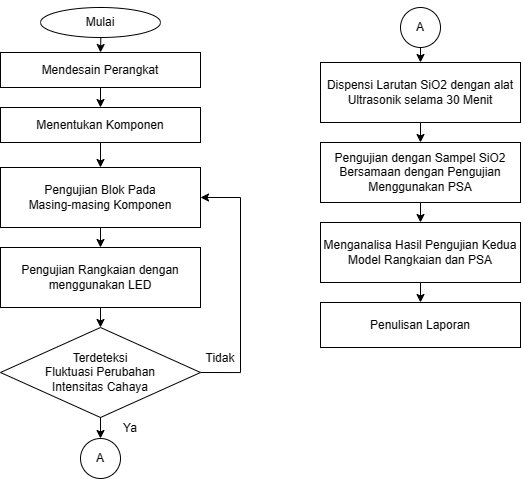
\includegraphics[width=12cm]{Images/Skema Penelitian.png}
    \caption{Diagram Alir Penelitian}
    \label{fig:reschart}
\end{figure}
\noindent Langkah-langkah pada gambar ~\ref{fig:reschart} dijelaskan sebagai berikut.

\begin{enumerate}
    \item Mendesain Perangkat agar dapat memastikan komponen yang dapat digunakan. Desain dari
    perangkat dibuat berdasarkan referensi yang didapatkan. Untuk membuat ruang gelap digunakan
    wadah hitam yang digunakan sebagai tempat pengukuran partikel dengan fotodioda. Untuk
    meminimalisir cahaya luar masuk ke sistem didalam ruang gelap, maka Arduino diposisikan
    di luar wadah.
    \item Menentukan Komponen. Berdasarkan desain yang telah dibuat, penentuan komponen dilakukan
    untuk menyesuaikan kebutuhan sesuai dengan spesifikasi yang dibutuhkan pada setiap proses
    pengambilan data. OPT101 digunakan sebagai fotodioda yang terintegrasi dengan
    \textit{Transimpedance Amplifier} sehingga tidak memerlukan Amplifier external sebagai filter
    aktif. Laser yang digunakan adalah modul laser merah 650nm dan modul laser hijau 532nm.
    \item Pengujian Blok pada Masing-masing komponen dilakukan untuk meminimalisir error yang
    dapat terjadi akibat dari salah satu komponen rangkaian. Setiap komponen diuji dengan
    menggunakan \textit{multimeter} dan \textit{power supply} untuk memastikan keluaran dari
    komponen.
    \item Rangkaian yang telah dirakit diuji dengan LED terlebih dahulu untuk memastikan
    apakah nilai keluaran sesuai dengan referensi. Nilai keluaran akan diproses dengan ADC
    \textit{(Analog Digital Converter)} dari sinyal pada sensor dan \textit{Transimpedance Amplifier}
    yang terdapat pada Arduino.
    \item Pengujian dengan sampel dilakukan bersamaan dengan pengujian pada PSA dari Horiba
    tipe SZ-100V2 pada ruangan
    dan suhu yang sama. Sampel yang digunakan merupakan ${SiO_2}$\cite{MadeJoni2020}
    berkarakteristik silika amorfus yang telah di ultrasonik selama 30 menit.
    \item Analisa Hasil Pengujian. Setelah didapatkan data dari kedua hasil pengujian, maka dilakukan
    analisa.
    \item Penulisan Laporan dilakukan sebagai bukti hasil yang didapat setelah melakukan penelitian.

\end{enumerate}


\section{Perancangan \textit{Prototype} Instrumen}

\subsection{Desain Sistem Instrumen DLS}

Rancangan dari rangkaian \textit{Dynamic Light Scattering} sederhana dengan dua laser yang
dibuat pada penelitian ini dapat digambarkan dengan Gambar ~\ref{fig:schemacirc}. Sistem dari
DLS dibuat dalam sebuah wadah tertutup gelap agar cahaya dari lingkungan tidak masuk kedalam
sistem. Laser merah dan Laser hijau diletakan menghadap kuvet, lalu diletakan stopper pada
salah satu sisi agar cahaya laser tidak terpantul kembali ke kuvet. Agar kedua laser dapat
digunakan bergantian, masing-masing laser dihubungkan dengan switch yang terhubung
dengan pin 5V dari arduino. Pada saat laser ditembakan ke kuvet, berkas cahaya laser yang
terhamburkan oleh partikel pada kuvet akan terdeteksi sensor fotodioda yang diletakan pada
sudut ${90\degree}$ dari sudut datang laser. Data yang diterima sensor lalu dikirim menuju Arduino
sebagai ADC dan diolah kembali pada program Python hingga didapatkan hasil pengukurannya.
\begin{figure}[H]
    \centering
    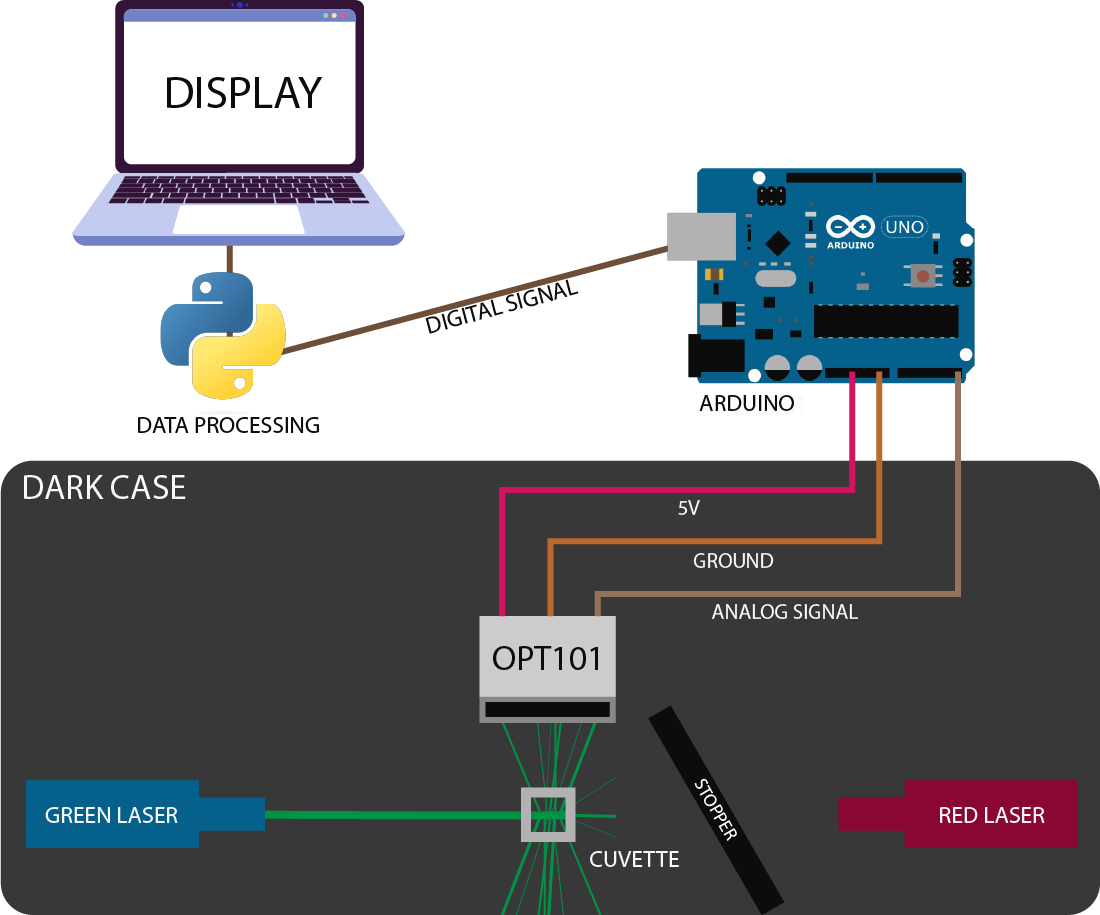
\includegraphics[width=14cm]{Images/Schema.png}
    \caption{Desain Rangkaian Instrumen DLS dua laser}
    \label{fig:schemacirc}
\end{figure}
\noindent
\textit{Transimpedance Amplifier} yang terdapat pada OPT101 dapat digambarkan dengan
diagram berikut yang bersumber dari datasheet \textit{Texas Instruments}
\begin{figure}[H]
    \centering
    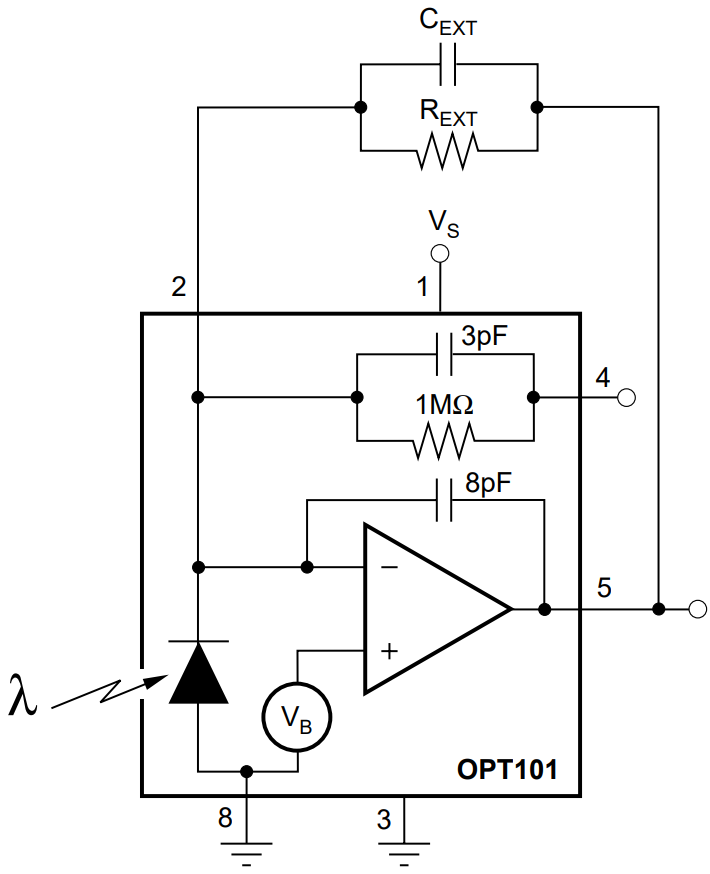
\includegraphics[width=8cm]{Images/Schema OPT101.png}
    \caption{Desain Rangkaian OPT101 (\textit{Texas Instruments})}
    \label{fig:schemaopt101}
\end{figure}
\noindent
Resistor Eksternal ${\left(R_{EXT} \right)}$ pada pengukuran partikel memiliki nilai
${10M \Omega}$ tanpa menggunakan Kapasitor Eksternal ${\left(C_{EXT}\right)}$. Namun untuk
memastikan pembesaran pada Amplifier sesuai, maka akan dilakukan
pengujian blok dengan variasi nilai Resistor Eksternal lainya.



\subsection{Diagram Blok Rangkaian}
\begin{figure}[H]
    \centering
    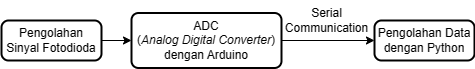
\includegraphics[width=12cm]{Images/Block Diagram.png}
    \caption{Diagram Blok Rangkaian DLS Sederhana}
    \label{fig:blockdiag}
\end{figure}

Diagram ~\ref{fig:blockdiag} dapat dijelaskan sebagai berikut.

\begin{enumerate}
    \item Pada instrumen DLS yang dibuat menggunakan fotodioda yang digunakan untuk mendeteksi
    hamburan cahaya dari pergerakan partikel. Fotodioda yang digunakan sudah terhubung dengan
    \textit{Transimpedance Amplifier} sehingga sinyal dari fotodioda dapat diperkuat untuk
    meningkatkan sensitivitas dari sensor tersebut.

    \item Sinyal yang keluar dari sistem fotodioda merupakan sinyal Analog sehingga untuk
    mengubahnya menjadi sinyal digital diperlukan ADC yang sudah terintegrasi pada Arduino.
    Sinyal dari Fotodioda terhubung dengan Arduino pada pin input A0.

    \item Sinyal yang telah diubah pada arduino disimpan, lalu dikirim menuju device seperti
    laptop. Device tersebut menerima data dengan serial communication
    dari Arduino. Data yang diterima akan diolah dengan program Python sehingga
    didapatkan nilai ukuran partikel.
\end{enumerate}


\subsection{Hasil Rancangan \textit{Prototype} Instrumen DLS}
Rangkaian DLS sederhana dua laser ini terdiri dari sebuah wadah \textit{casing} berbentuk balok
yang terbuat dari \textit{polymer} berwarna hitam dengan dimensi ${21.5 \times }$
${14.5 \times 8.5cm}$. Untuk mengurangi cahaya luar masuk ke sistem fotodioda digunakan sekat
yang membatasi kuvet dengan laser. Hasil rancangan alat tersebut dapat dilihat pada gambar
~\ref{fig:prot}.
\begin{figure}[H]
    \centering
    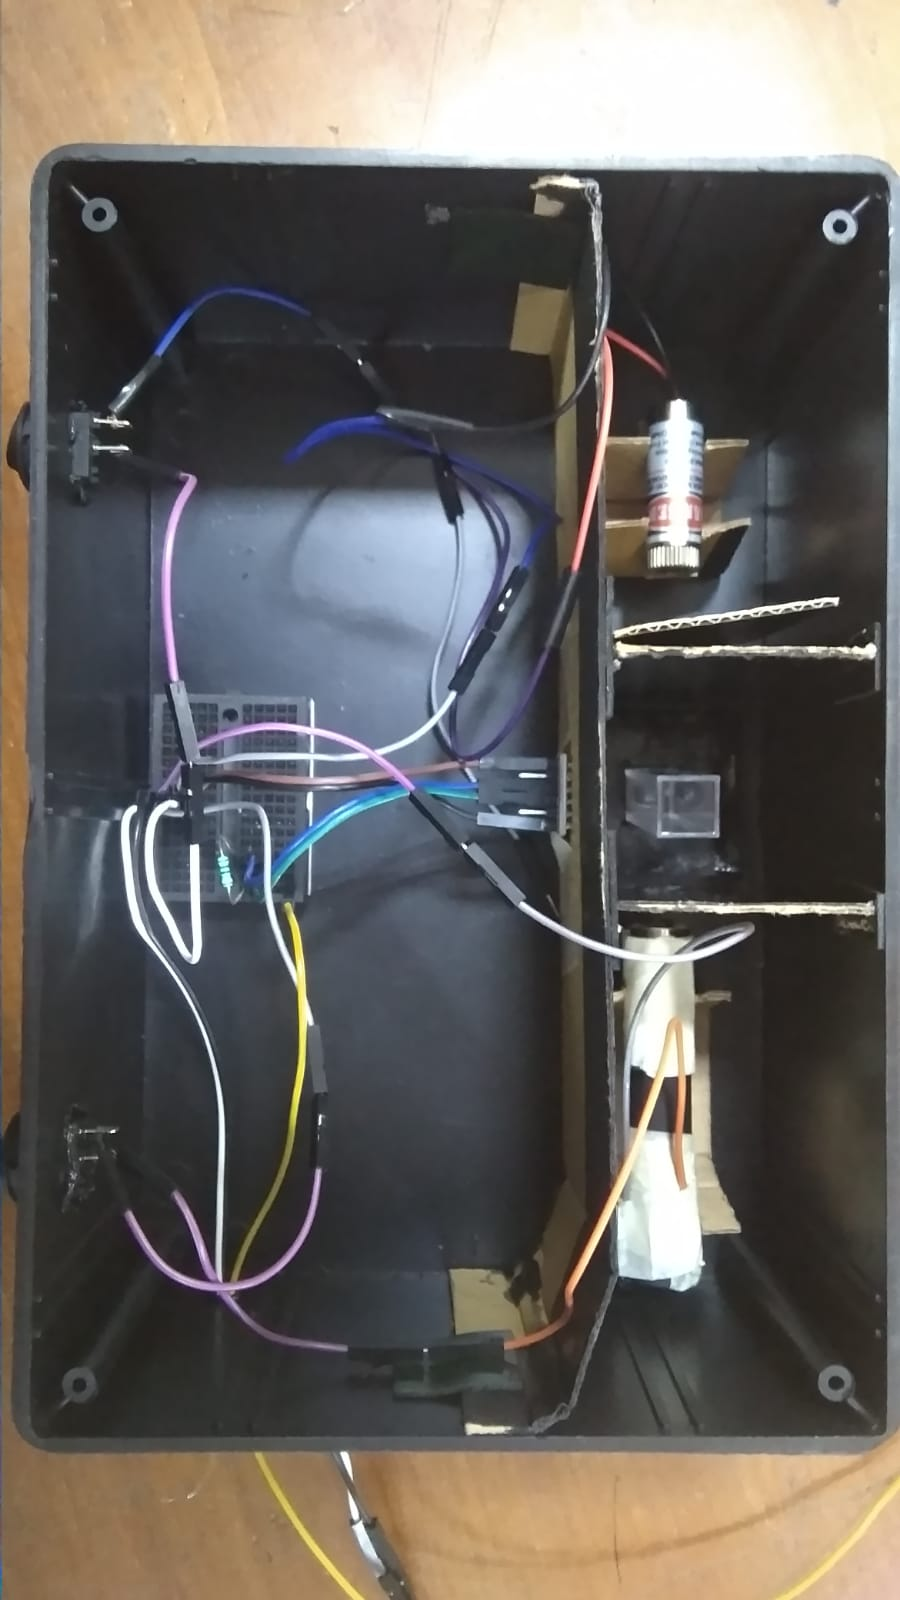
\includegraphics[width=12cm]{Images/Rangkaian.jpg}
    \caption{\textit{Prototype} Instrumen DLS Sederhana Dua Laser}
    \label{fig:prot}
\end{figure}

\noindent
Untuk menggunakan laser secara bergantian, setiap laser dihubungkan dengan switch
sehingga pada saat salah satu laser digunakan, laser lainnya dapat dimatikan untuk
mengurangi cahaya lingkungan masuk ke sistem.



\section{Desain Software}

\subsection{Pengolahan Data pada Arduino}
Penjelasan sistematika pengolahan data sensor pada arduino digambarkan pada gambar
~\ref{fig:schemaard}

\begin{figure}[H]
    \centering
    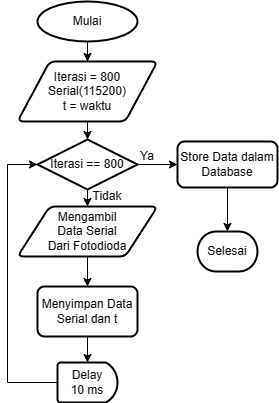
\includegraphics[width=8cm]{Images/Skema Arduino.png}
    \caption{Skema Pengolahan Data pada Arduino}
    \label{fig:schemaard}
\end{figure}
Sinyal yang keluar dari rangkaian fotodioda dan \textit{Transimpedance Amplifier} masuk melalui
pin input A0 Arduino. Sinyal tersebut diolah menjadi sinyal digital sehingga dapat dibaca dalam
bentuk angka pada komputer. Kecepatan pembacaan data dari sensor diatur dengan serial Arduino
yang pada penelitian ini optimumnya menggunakan \textit{baudrate} 115200. Spesifikasi dari
Arduino Uno R3 memiliki kapasitas penyimpanan dalam satu iterasi kurang lebih sebanyak 800
data dan akan dibangun dalam bentuk \textit{array}. Durasi iterasi penyimpanan data ditetapkan
sebagai variabel ${t}$.



\subsection{Pengolahan Data pada Python}
Ketika Arduino terhubung dengan laptop atau perangkat pengolahan data, setiap iterasi akan diolah
oleh program Python. Dengan menggunakan library \textit{Serial Communication}, pengiriman data
akan berjalan secara otomatis selama Arduino terhubung dengan laptop. Pengolahan data yang
diterima oleh laptop dapat digambarkan pada gambar ~\ref{fig:schemapy}

\begin{figure}[H]
    \centering
    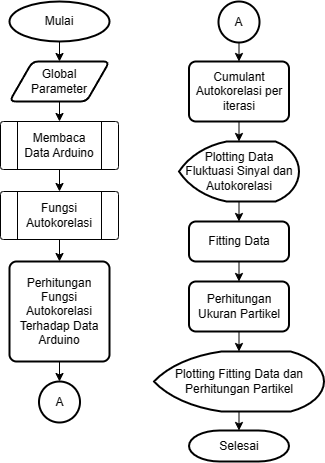
\includegraphics[width=9cm]{Images/Skema Python.png}
    \caption{Skema Pengolahan Data pada Python}
    \label{fig:schemapy}
\end{figure}

Data yang diterima program Python berupa 800 nilai dari pembacaan sensor dalam waktu ${t}$
didefinisikan sebagai \textit{Global Parameter}. Selain itu terdapat nilai Panjang gelombang
Laser, Indeks Bias, Konstanta Boltzman, Suhu sampel, Viskositas Sampel, dan Sudut Hamburan.
Nilai sensor yang dikirim melalui Serial akan diolah menggunakan Metode Kumulan Autokorelasi
dengan menggunakan \textit{numpy corelate}. Dalam persamaan matematis, Fungsi Autokorelasi
dapat dituliskan sebagai berikut:
\begin{equation}
    \hat{\gamma} = \frac{1}{n} \sum_{t=1}^{n-k}\left(y_t - \bar{y}\right)\left(y_{t+k} - \bar{y}\right)
\end{equation}
\noindent
dengan aturan fungsi ini dijalankan hingga nilai ${k}$ dimana ${k}$ sama dengan ${n-1}$

Data hasil autokorelasi tersebut tersimpan dalam bentuk
\textit{array}, lalu di plotting sehingga dapat dilakukan fitting data untuk mencari nilai
${c}$ yang mengacu pada persamaan~\ref{eq:c}. Kemudian perhitungan ukuran partikel
dilakukan dengan persamaan~\ref{eq:rh} untuk mencari nilai jari-jari partikel
berdasarkan nilai ${c}$.


\section{Pengambilan Data}
Pengujian alat dilakukan dengan menggunakan sampel \textit{Silika Geothermal} (${SiO_2}$)
\cite{MadeJoni2020} berkarakteristik silika amorfus yang dipanaskan dengan suhu rendah
(${70\degree C - 90\degree C}$) yang
telah di ultrasonik selama 30 menit agar distribusi ukuran partikel dalam pelarut homogen.
Pengambilan data dari DLS sederhana dilakukan bersamaan dengan karakterisasi menggunakan PSA
pada suhu ruangan (${20\degree C}$).

\subsection{Pengukuran dengan DLS Sederhana}
Data yang disimpan pada Arduino merupakan fluktuasi intensitas hamburan cahaya yang terdeteksi
pada sensor terhadap waktu. Data tersebut dijadikan variabel untuk perhitungan autokorelasi
hingga perhitungan ukuran partikel. Pengujian pada setiap laser dilakukan secara bergantian.
Untuk memastikan bahwa perhitungan pada program sesuai, data awal dari sensor disimpan dalam
penyimpanan lokal.

Pengambilan data ukuran partikel dilakukan sebanyak 10.000 kali untuk setiap laser. Total data
ukuran partikel berjumlah 20.000. Semua data yang terkumpul tercatat sebagai distribusi
ukuran partikel untuk masing-masing laser.

\subsection{Karakterisasi Sampel dengan PSA}
Pada waktu yang sama dilakukan karakterisasi psa untuk mengetahui distribusi ukuran partikel
sampel sebagai dasar untuk menganalisa kesesuaian data yang didapatkan dari DLS sederhana.
Data keluaran dari PSA berupa distribusi ukuran partikel dan \textit{Z-average} dari sampel
tersebut.